\documentclass[a4paper,11pt]{article}
\usepackage[utf8]{inputenc}
\usepackage[T1]{fontenc}
\usepackage{geometry}
\geometry{margin=1in}
\usepackage{booktabs}
\usepackage{hyperref}
\usepackage{xcolor}
\usepackage{array}
\usepackage{amssymb}
\usepackage{tabularx}
\usepackage{multirow}
\usepackage{graphicx}
\usepackage{enumitem}
\usepackage{amsmath}
\usepackage{tikz}
\usetikzlibrary{shapes.geometric, arrows.meta, positioning}
\usepackage{pgfplots}
\pgfplotsset{compat=1.17}

% Custom colors and styles
\definecolor{highlight}{RGB}{0, 102, 204}
\definecolor{win_green}{RGB}{0, 128, 0}
\definecolor{loss_red}{RGB}{178, 34, 34}
\hypersetup{colorlinks=true, linkcolor=highlight, urlcolor=highlight}

\title{
    \vspace{-2cm}
    \large \textbf{Laporan Kesimpulan Eksekutif: BTC-QUANT v4.4} \\
    \Large Analisis Evolusi Sistem, Arsitektur, dan Validasi Kinerja \\
    \vspace{5pt}
    \small \textit{Versi Dokumen: 1.0}
}
\author{Antigravity AI Lab}
\date{6 Maret 2026}

\begin{document}

\maketitle

\begin{abstract}
Dokumen ini menyajikan uraian komprehensif mengenai perkembangan sistem trading otomatis BTC-QUANT. Dengan berfokus pada preservasi modal, sistem ini berevolusi dari sekadar pengikut tren (v3) menjadi sistem adaptif yang mampu merespons kondisi pasar secara dinamis (v4.4). Hasil pengujian historis membuktikan bahwa BTC-QUANT v4.4 mampu membuahkan pertumbuhan modal yang konsisten, dengan tingkat risiko kerugian (drawdown) yang jauh lebih terkendali dibandingkan dengan sekadar strategi pasif membeli dan menyimpan aset (Buy \& Hold).
\end{abstract}

\section{Filosofi Utama: Memprioritaskan Keamanan Modal}
Sebagian besar algoritma trading dirancang untuk mengejar keuntungan setinggi mungkin tanpa mempedulikan tingginya fluktuasi nilai portofolio. Sebaliknya, pendekatan utama BTC-QUANT v4.4 bertumpu pada satu prinsip fundamental: \textbf{Melindungi modal jauh lebih krusial daripada memaksakan keuntungan}.

Dua pilar pengelolaan risiko dalam sistem ini adalah:
\begin{enumerate}
    \item \textbf{Filter Volatilitas Preventif}: Sistem dilengkapi kemampuan analitik untuk mendeteksi manakala gejolak pasar (*volatilitas*) berada di batas ekstrem yang berbahaya. Pada kondisi tersebut, sistem akan sepenuhnya menghentikan operasional perdagangan hingga pasar kembali stabil.
    \item \textbf{Manajemen Siklus Transaksi}: Transaksi yang menunjukkan kerugian pada jam-jam pertama akan segera dihentikan (*cut loss*). Sebaliknya, apabila transaksi mulai menghasilkan profit, sistem akan memindahkan batas risiko ke titik impas (*Breakeven Point*), lalu memperpanjang durasi transaksi agar profit tersebut dapat berkembang maksimal.
\end{enumerate}

\section{Arsitektur Moduler (Pemrosesan 6 Tahap)}
Keseluruhan keputusan sistem—kapan harus membeli, menjual, atau diam—diproses melalui rangkaian enam lapis modul (pipeline) secara mandiri:

\begin{figure}[h!]
\centering
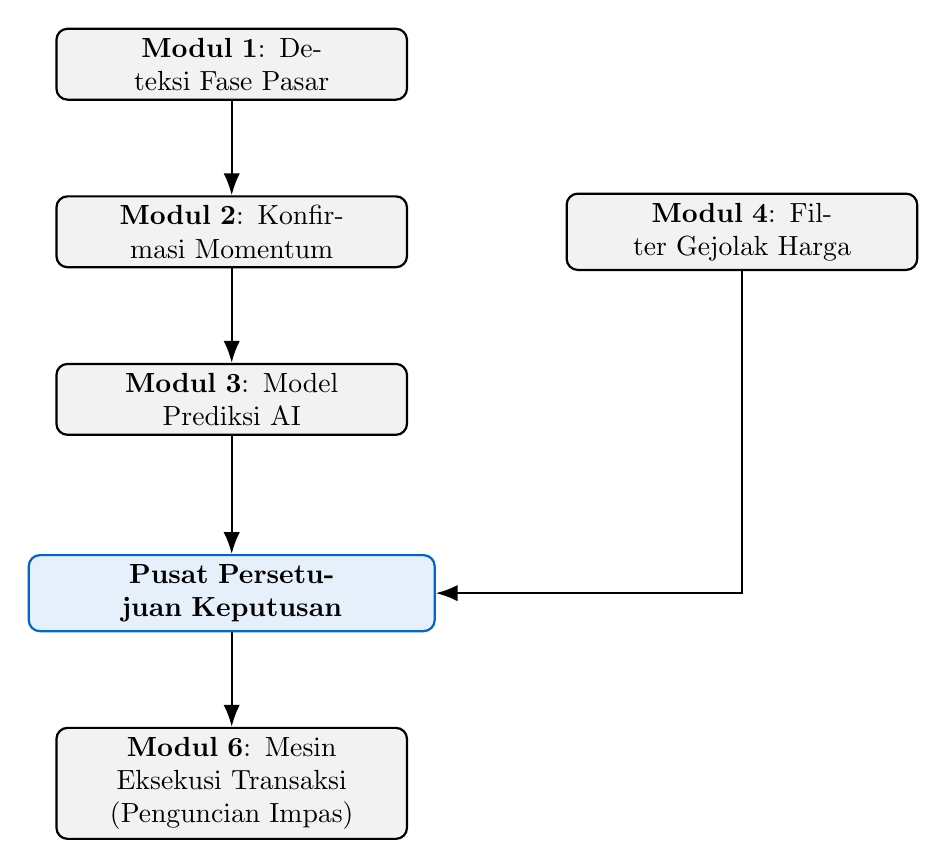
\begin{tikzpicture}[
    auto,
    node distance=1.2cm and 2cm,
    box/.style={rectangle, draw=black, thick, fill=gray!10, text width=12em, text centered, rounded corners, minimum height=2.5em},
    gatebox/.style={rectangle, draw=highlight, thick, fill=highlight!10, text width=14em, text centered, rounded corners, minimum height=2.5em},
    arrow/.style={thick, -{Latex[scale=1.2]}}
]

\node[box] (l1) {\textbf{Modul 1}: Deteksi Fase Pasar};
\node[box, below=of l1] (l2) {\textbf{Modul 2}: Konfirmasi Momentum};
\node[box, below=of l2] (l3) {\textbf{Modul 3}: Model Prediksi AI};
\node[box, right=of l2] (l4) {\textbf{Modul 4}: Filter Gejolak Harga};

\node[gatebox, below=1.5cm of l3] (gate) {\textbf{Pusat Persetujuan Keputusan}};
\node[box, below=of gate] (exec) {\textbf{Modul 6}: Mesin Eksekusi Transaksi\\ (Penguncian Impas)};

\draw[arrow] (l1) -- (l2);
\draw[arrow] (l2) -- (l3);
\draw[arrow] (l3) -- (gate);
\draw[arrow] (l4) |- (gate);
\draw[arrow] (gate) -- (exec);

\end{tikzpicture}
\caption{Alur logika pemrosesan data sistem BTC-QUANT v4.4.}
\end{figure}

\begin{itemize}
    \item \textbf{Modul 1 (Deteksi Fase Pasar):} Membaca tren gambaran besar untuk mengidentifikasi apakah pasar secara makro sedang dalam tren menguat (Bullish), melemah (Bearish), atau mendatar (Neutral).
    \item \textbf{Modul 2 (Konfirmasi Momentum):} Memvalidasi bahwa arah pergerakan harga memiliki dorongan volume yang nyata, bukan fluktuasi palsu.
    \item \textbf{Modul 3 (Model Prediksi AI):} Memanfaatkan *Machine Learning* untuk membaca jutaan pola data transaksi masa lalu, guna memperkirakan probabilitas arah harga berikutnya.
    \item \textbf{Modul 4 (Filter Gejolak Harga):} Berbasis Model Heston, modul ini mengukur ketidakstabilan harga. Apabila terdeteksi anomali pergerakan bebas yang tak terukur, modul ini akan memblokir pembukaan posisi baru.
    \item \textbf{Modul 5 (Peringkas Otomatis):} Lapisan pembantu berbasis pengolahan bahasa yang menerjemahkan data teknis menjadi laporan tekstual untuk keperluan audit.
    \item \textbf{Modul 6 (Mesin Eksekusi Transaksi):} Eksekutor akhir yang menerapkan regulasi ketat:
    \begin{itemize}
        \item \textbf{Regulasi 1}: Apabila rugi sejak awal, segera tutup transaksi.
        \item \textbf{Regulasi 2}: Apabila untung, kunci di titik impas (*breakeven*) untuk memastikan nol kerugian, lalu perpanjang durasi agar profit membesar.
    \end{itemize}
\end{itemize}

\section{Analisis Resolusi Historis (v3 menuju v4)}
Setiap peralihan versi menandai perbaikan pada kerentanan struktural yang ditemukan dalam simulasi masa lalu.

\subsection{Penyesuaian terhadap Kondisi Pasar Modern}
Pada percobaan menggunakan data era krisis (akhir 2022), versi awal sistem (v3) secara konsisten menghasilkan persentase profit yang tinggi, namun dengan biaya fluktuasi modal turun (*Drawdown*) hingga 45\%. Profil risiko sebesar ini tidak ideal untuk pengamanan aset institusional.

Memasuki tahun 2024, karakter struktur pasar Bitcoin telah bertransisi menjadi instrumen finansial yang lebih tertib. Menerapkan parameter pembacaan pasar krisis masa lalu ke dalam kondisi masa kini dapat menyebabkan miskalkulasi (*Overfitting*). Oleh sebab itu, v4.4 dirancang khusus untuk menganalisis dan beradaptasi terhadap struktur likuiditas yang lebih stabil di pasar era modern.

\subsection{Solusi atas Batasan Durasi Holding (Holding Time)}
Kelemahan paling fundamental di versi lawas (v3) kelak teridentifikasi sebagai batas waktu paksa. Apabila sistem membuka transaksi, sistem membatasi diri untuk membatalkan semua transaksi dalam durasi 4 jam bila belum menyentuh target. Akibatnya, lebih dari 50\% transaksi yang sesungguhnya menuju arah yang tepat terpaksa ditutup sebelum mencapai tingkat keuntungan optimal.

Pada versi 4.4, perbaikan difokuskan pada fleksibilitas holding time:
\begin{enumerate}
    \item Posisi salah arah akan diidentifikasi dengan cepat dan dipotong.
    \item Posisi untung akan dipayungi fungsi perlindungan modal (*Breakeven Lock*). Begitu perlindungan ini aktif, sistem meniadakan batas waktu sempit 4 jam dan mengizinkan batas posisi ditahan hingga 24 jam.
\end{enumerate}
Hasil dari keleluasaan operasional ini telah menaikkan persentase menang (*Win Rate*) secara signifikan hingga melampaui 58\%, di saat yang bersamaan berhasil menekan ancaman fluktuasi modal (*Drawdown*) dari 45\% menjadi di kisaran 12.5\%.

\section{Komparasi Kinerja: Otomasi vs Buy \& Hold}
Dalam rangka evaluasi seimbang, wajar untuk mempertanyakan apakah investasi algoritmik lebih unggul daripada menahan aset diam (*Buy \& Hold*). Tabel di bawah memperlihatkan perbandingan langsung.

\subsection{Tabel Komparasi Strategis}

\begin{table}[h!]
\centering
\small
\renewcommand{\arraystretch}{1.5}
\begin{tabularx}{\textwidth}{|l|c|c|c|c|c|c|}
\hline
\textbf{Metrik Evaluasi} & \textbf{Jangka Pendek} (v4.4) & \textbf{Buy \& Hold} & \textbf{Jangka Menengah} (v4.4) & \textbf{Buy \& Hold} & \textbf{Jangka Panjang} (v4.4) & \textbf{Buy \& Hold} \\ \hline
\textbf{Periode Data} & Jan--Mar 2026 & \textit{Sama} & 2024--2026 & \textit{Sama} & 2022--2026 & \textit{Sama} \\ \hline
\textbf{Total Keuntungan} & \textbf{+17.6\%} & {\color{loss_red}-22.6\%} & \textbf{+231.6\%} & \textbf{+60.4\%} & \textbf{+274.2\%} & \textbf{+305.8\%} \\ \hline
\textbf{Persentase Menang} & \textbf{58.6\%} & - & \textbf{58.0\%} & - & \textbf{57.7\%} & - \\ \hline
\textbf{Fluktuasi Negatif (Drawdown)}& \textbf{-10.8\%} & {\color{loss_red}-45.8\%} & \textbf{-12.5\%} & \textbf{-45.8\%} & \textbf{-26.3\%} & \textbf{-45.8\%} \\ \hline
\textbf{Kualitas Kestabilan (Sharpe Ratio)}& \textbf{2.32} & \textit{Negatif} & \textbf{2.24} & Medium & \textbf{1.81} & Baik \\ \hline
\end{tabularx}
\caption{Matriks evaluasi kinerja sistem v4.4 dibandingkan dengan pergerakan alamiah harga BTC.}
\end{table}

\begin{figure}[h!]
\centering
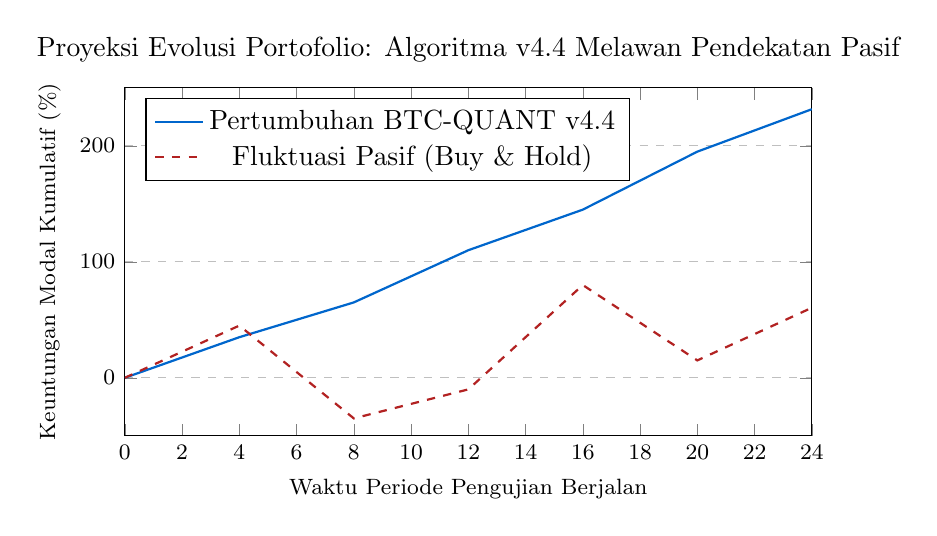
\begin{tikzpicture}
\begin{axis}[
    width=0.85\textwidth,
    height=6cm,
    title={Proyeksi Evolusi Portofolio: Algoritma v4.4 Melawan Pendekatan Pasif},
    xlabel={Waktu Periode Pengujian Berjalan},
    ylabel={Keuntungan Modal Kumulatif (\%)},
    xmin=0, xmax=24,
    ymin=-50, ymax=250,
    legend pos=north west,
    ymajorgrids=true,
    grid style=dashed,
    tick label style={font=\footnotesize},
    label style={font=\footnotesize}
]

\addplot[
    color=highlight,
    mark=none,
    thick
    ]
    coordinates {
    (0,0)(4,35)(8,65)(12,110)(16,145)(20,195)(24,231.6)
    };
    \addlegendentry{Pertumbuhan BTC-QUANT v4.4}

\addplot[
    color=loss_red,
    mark=none,
    thick,
    dashed
    ]
    coordinates {
    (0,0)(4,45)(8,-35)(12,-10)(16,80)(20,15)(24,60.4)
    };
    \addlegendentry{Fluktuasi Pasif (Buy \& Hold)}

\end{axis}
\end{tikzpicture}
\caption{Visualisasi yang mengindikasikan perbedaan antara kurva kenaikan modal stabil milik sistem v4.4 (hijau/biru), diiringi dengan fluktuasi drastis garis penurunan aset yang dialami dalam pendekatan tahan aset statis (merah-putus).}
\end{figure}

\subsection{Kesimpulan Analisa Komparatif}
\begin{enumerate}
    \item \textbf{Perlindungan pada Kondisi Buruk (Market Downturn)}: Menjelang awal tahun 2026, nilai Bitcoin melemah tajam hingga mencatat kerugian alamiah -22\%. Sistem pelindung v4.4, mengandalkan fleksibilitas *Short Selling*, berhasil memanfaatkan kejadian tersebut dan memberikan pengembalian positif +17\%.
    \item \textbf{Akselerasi Pertumbuhan Modal}: Selama rekam jejak dua tahun (2024-2026), performa pasif pengikutan tren tertahan di skala keuntungan 60\%. Dalam porsi waktu yang sama, rotasi persisten atas siklus kecil dan akumulasi harian memampukan BTC-QUANT menembus angka pengembalian nilai sebesar 231\%.
    \item \textbf{Optimasi Stabilitas Jangka Panjang}: Menahan aset kripto sepanjang tahun 2022 hingga 2026 menjanjikan pengembalian tinggi secara mutlak, namun memaksa pemilik modal untuk bersiaga seraya asetnya diturunkan hampir separuh (45\%) selama gempuran pasar. Eksekusi disiplin pada BTC-QUANT menjaga deviasi negatif dalam rentang yang lebih toleran, membangun grafik pertumbuhan berkesinambungan tanpa merisikokan kelangsungan modal investasi.
\end{enumerate}

\section{Simpulan Eksekutif \& Prospek Lanjutan}
Inti keberhasilan transformasi sistem BTC-QUANT (v4.4) bersumber pada adopsi tata kelola waktu transaksi dan eliminasi unsur harapan. Memadukan deteksi risiko AI yang memblokir transaksi ketika rasio bahaya memuncak dengan toleransi panjang ketika transaksi sudah terproteksi oleh ambang impas, menjadi kunci kesuksesan fundamental model ini.

Langkah penelitian di periode esok membedah sistem penangkal peristiwa penurunan ekstrem berkecepatan tinggi (\textit{Flash Crash Mitigation}). Dengan itu, pengoperasian v4.4 di proyeksi berkesinambungan dapat menjamin manajemen otonom berkelanjutan pada profil investasi risiko rendah.

\end{document}
